\documentclass{standalone}
\usepackage{tikz}
\usetikzlibrary{patterns}

\tikzset{
  svgfrag/.style 2 args={
    execute at begin scope={\special{dvisvgm:raw <g class="fragment #2" data-fragment-index="#1">}},
    execute at end scope={\special{dvisvgm:raw </g>}},
    execute at begin node={\special{dvisvgm:raw <g class="fragment #2" data-fragment-index="#1">}},
    execute at end node={\special{dvisvgm:raw </g>}},
  }
}

\begin{document}
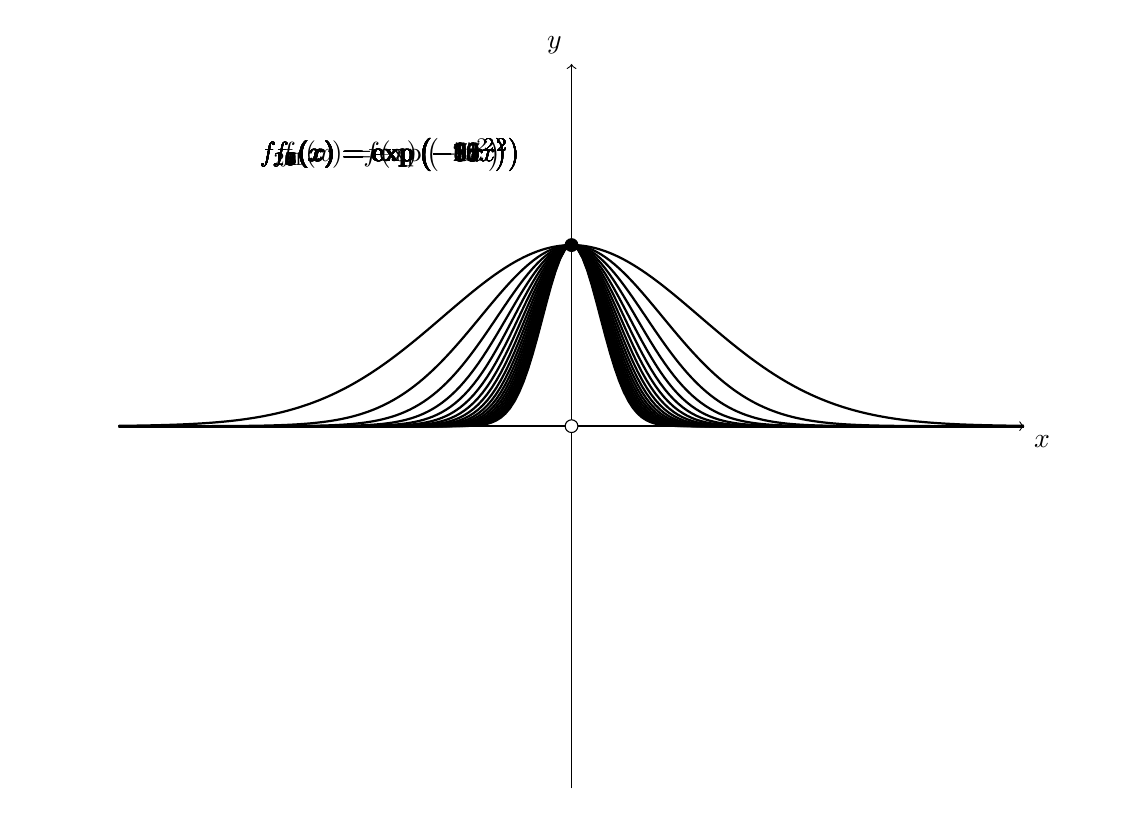
\begin{tikzpicture}[scale=2.3]
    \draw[white] (-3,-2.1) rectangle (3,2.1);
    \draw[thin, ->] (-2.5,0) -- (2.5,0)node[below right]{$x$};
    \draw[thin, ->] (0, -2) -- (0, 2)node[above left]{$y$};
    \begin{scope}[svgfrag={1}{fade-in-then-out}]
        \clip (-2.5,-2) rectangle (2.5, 2);
        \draw[thick, domain=-2.5:2.5] plot[samples=200] (\x, {exp(-(\x)^2)});
        \node at (-1, 1.5) {$f_1(x) = \exp\left(-x^2\right)$};
    \end{scope}
    \foreach \i in {2,...,20}{
        \begin{scope}[svgfrag={\i}{fade-in-then-out}]
            \clip (-2.5,-2) rectangle (2.5, 2);
            \draw[thick, domain=-2.5:2.5] plot[samples=200] (\x, {exp(-\i*(\x)^2});
            \node at (-1, 1.5) {$f_{\i}(x) = \exp\left(-\i x^2\right)$};
        \end{scope}
    }
    \begin{scope}[svgfrag={21}{fade-in}]
        \clip (-2.5,-2) rectangle (2.5, 2);
        \draw[thick] (-2.5,0) -- (2.5,0);
        \draw[fill] (0,1) circle[radius=1pt];
        \draw[fill=white] (0,0) circle[radius=1pt];
        \node at (-1, 1.5) {$f(x)$};
    \end{scope}
\end{tikzpicture}
\end{document}
